\section{Numerical solutions in the low frequency limit}
In this section we numerically solve the linear stability problem.  
We relax the thin-disk assumption, using the full, non-Keplerian
expressions of $\rho$, $\Omega$ and $\kappa$, so that we may consider
vertical domains up to $z\sim r$. However, we retain the low-frequency
approximation $|\sigma^2|\ll\kappa^2$ to obtain a linear eigenvalue
problem, which limits us to consider large radial wavenumbers
$k_x$. We will relax this in the next section when considering
moderate values of $k_x$. % This level of approximation lies in between
% the full problem Eq. \ref{iso_ode}, solved by \cite{mcnally14}, and
% the thin-disk limit Eq. \ref{iso_ode3}, solved by \cite{nelson13}.    


%We will solve different versions of the linearized equations depending
%on the disk properties, but in all cases we use 

\subsection{Vertically isothermal disks with isothermal perturbations}   
We first validate the low-frequency approximation by re-producing
results from \cite{mcnally14} who solved the full problem for
vertically isothermal disks ($\Gamma=1$) subject to isothermal
perturbations ($\gamma=1$). The parameters are $q=-1$,
$p=-1.5$, $\epsilon=0.1$ and $k_x = 200\pi/r$ (or $\hat{k} = 20\pi$),
with solid vertical boundaries. 

For this problem we solve Eq. \ref{iso_ode}, with $D$ replaced by
$\kappa^2$, using a pseudo-spectral
method by expanding $W$ in Chebyshev polynomials $T_l$ up to $l=512$
and discretizing the equation on a grid with
$\zmax=10H_\mathrm{iso}$. This procedure converts the linear problem
to a standard matrix eigenvalue problem.   

Fig. \ref{lowfreq_eigen} shows the eigenvalues $\sigma = \omega +
\ii\nu$. This plot is effectively identical to that in
\cite{mcnally14}. The fundamental VSI mode, with one node in $W$, has
the smallest $|\sigma|$ and is shown in Fig. \ref{lowfreq_eigenfunc}.  
The expected growth rate from Eq. \ref{simple_growth} with 
$L=1$ is  
\begin{align*}
  \nu = 0.2606\epsilon\Omega_k,
\end{align*}
as obtained numerically. This agreement is surpsingly good, given that
Eq. \ref{simple_growth} assumes the thin-disk approximation and
imposes a different boundary condition to that in the numerical
calculation. The eigenfunction $W$ is qualitatively proportional to
$z$, as expected for the fundamental mode according to explicit
solutions discussed in \S\ref{iso_poly}.    

\begin{figure}
  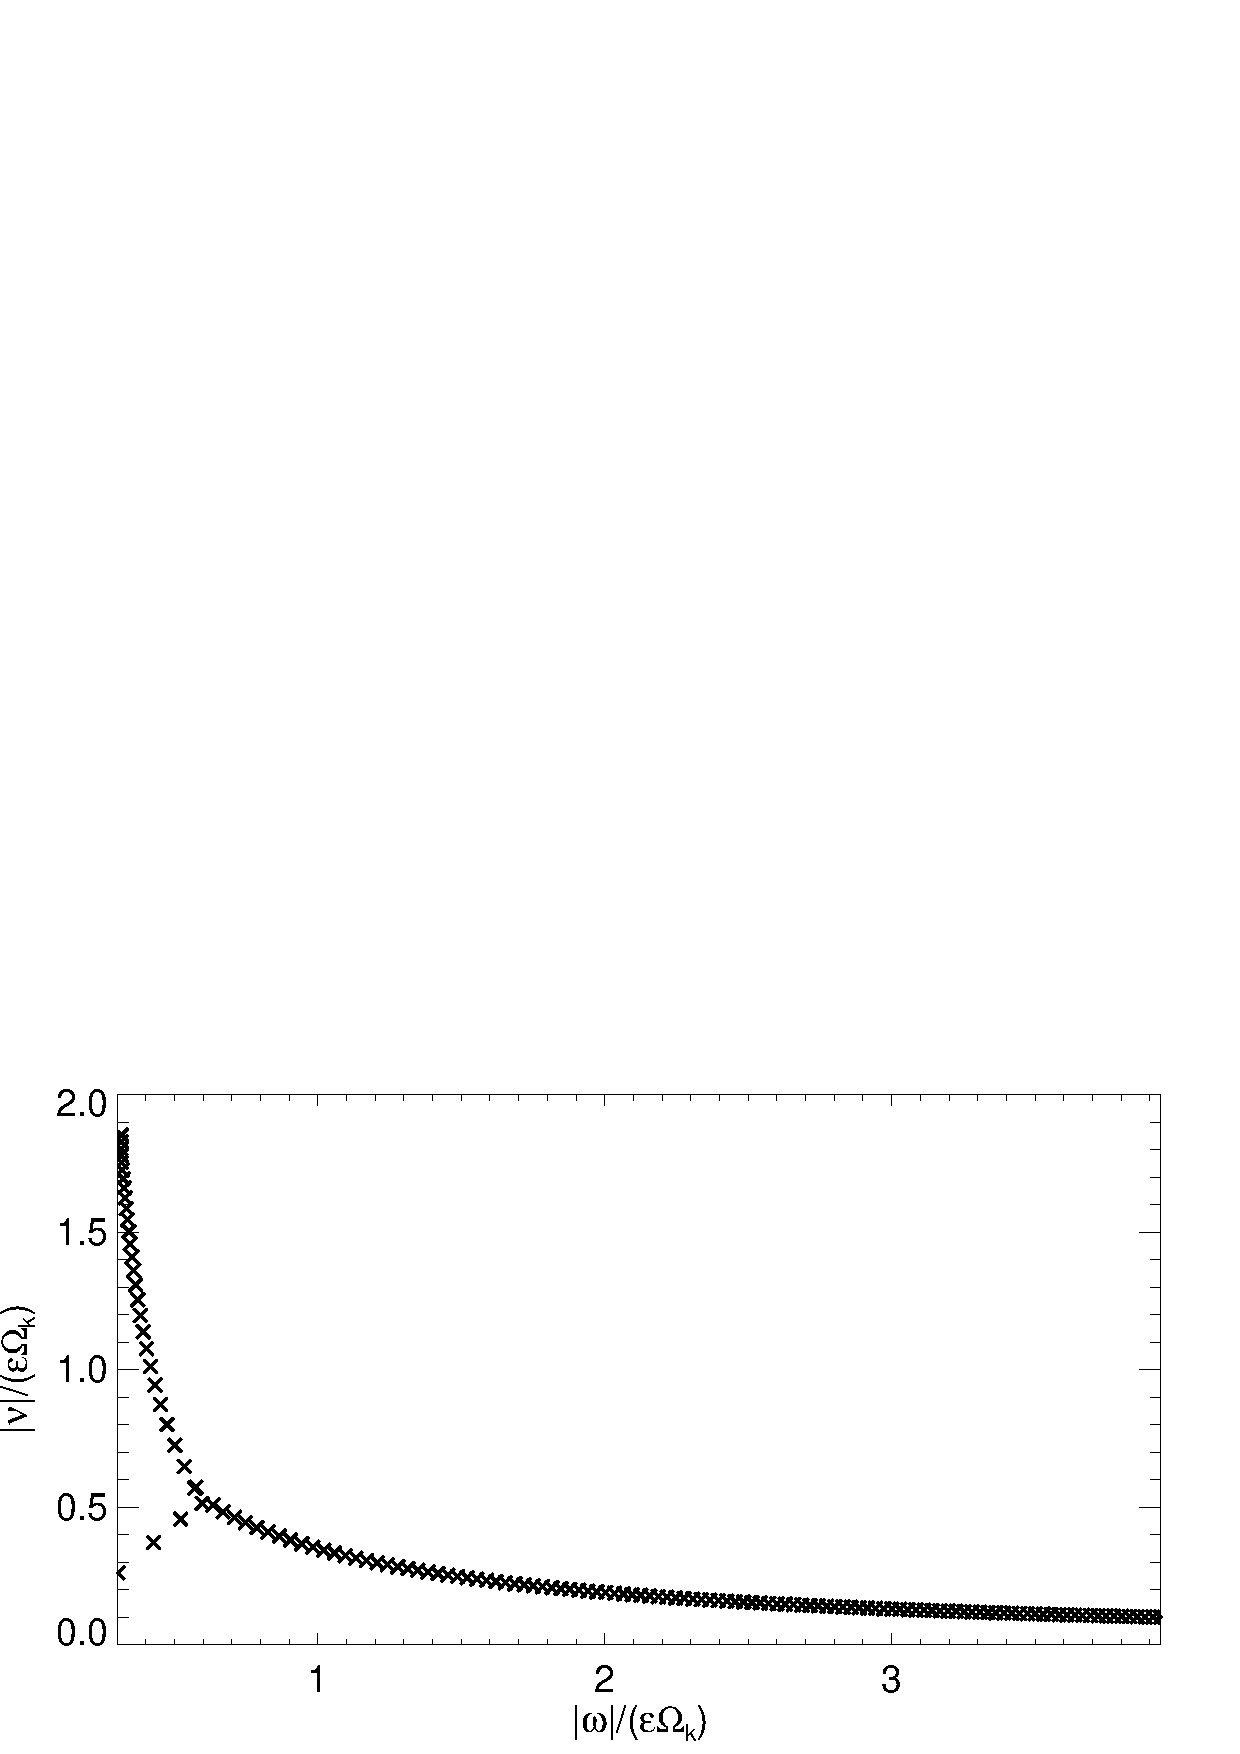
\includegraphics[width=\linewidth]{figures/eigenvalues_iso}
  \caption{Eigenvalues in the low-frequency approximation for the
    vertical shear instability in a vertically isothermal disk evolved
    isothermally ($\gamma=\Gamma=1$). The disk parameters are $q=-1$,
    $p=-1.5$ and $\epsilon=0.1$, while the perturbation radial
    wavenumber is $k_x=200\pi/r$. This is the set up considered in
    \cite{mcnally14}. \label{lowfreq_eigen}
  }
\end{figure}

\begin{figure}
  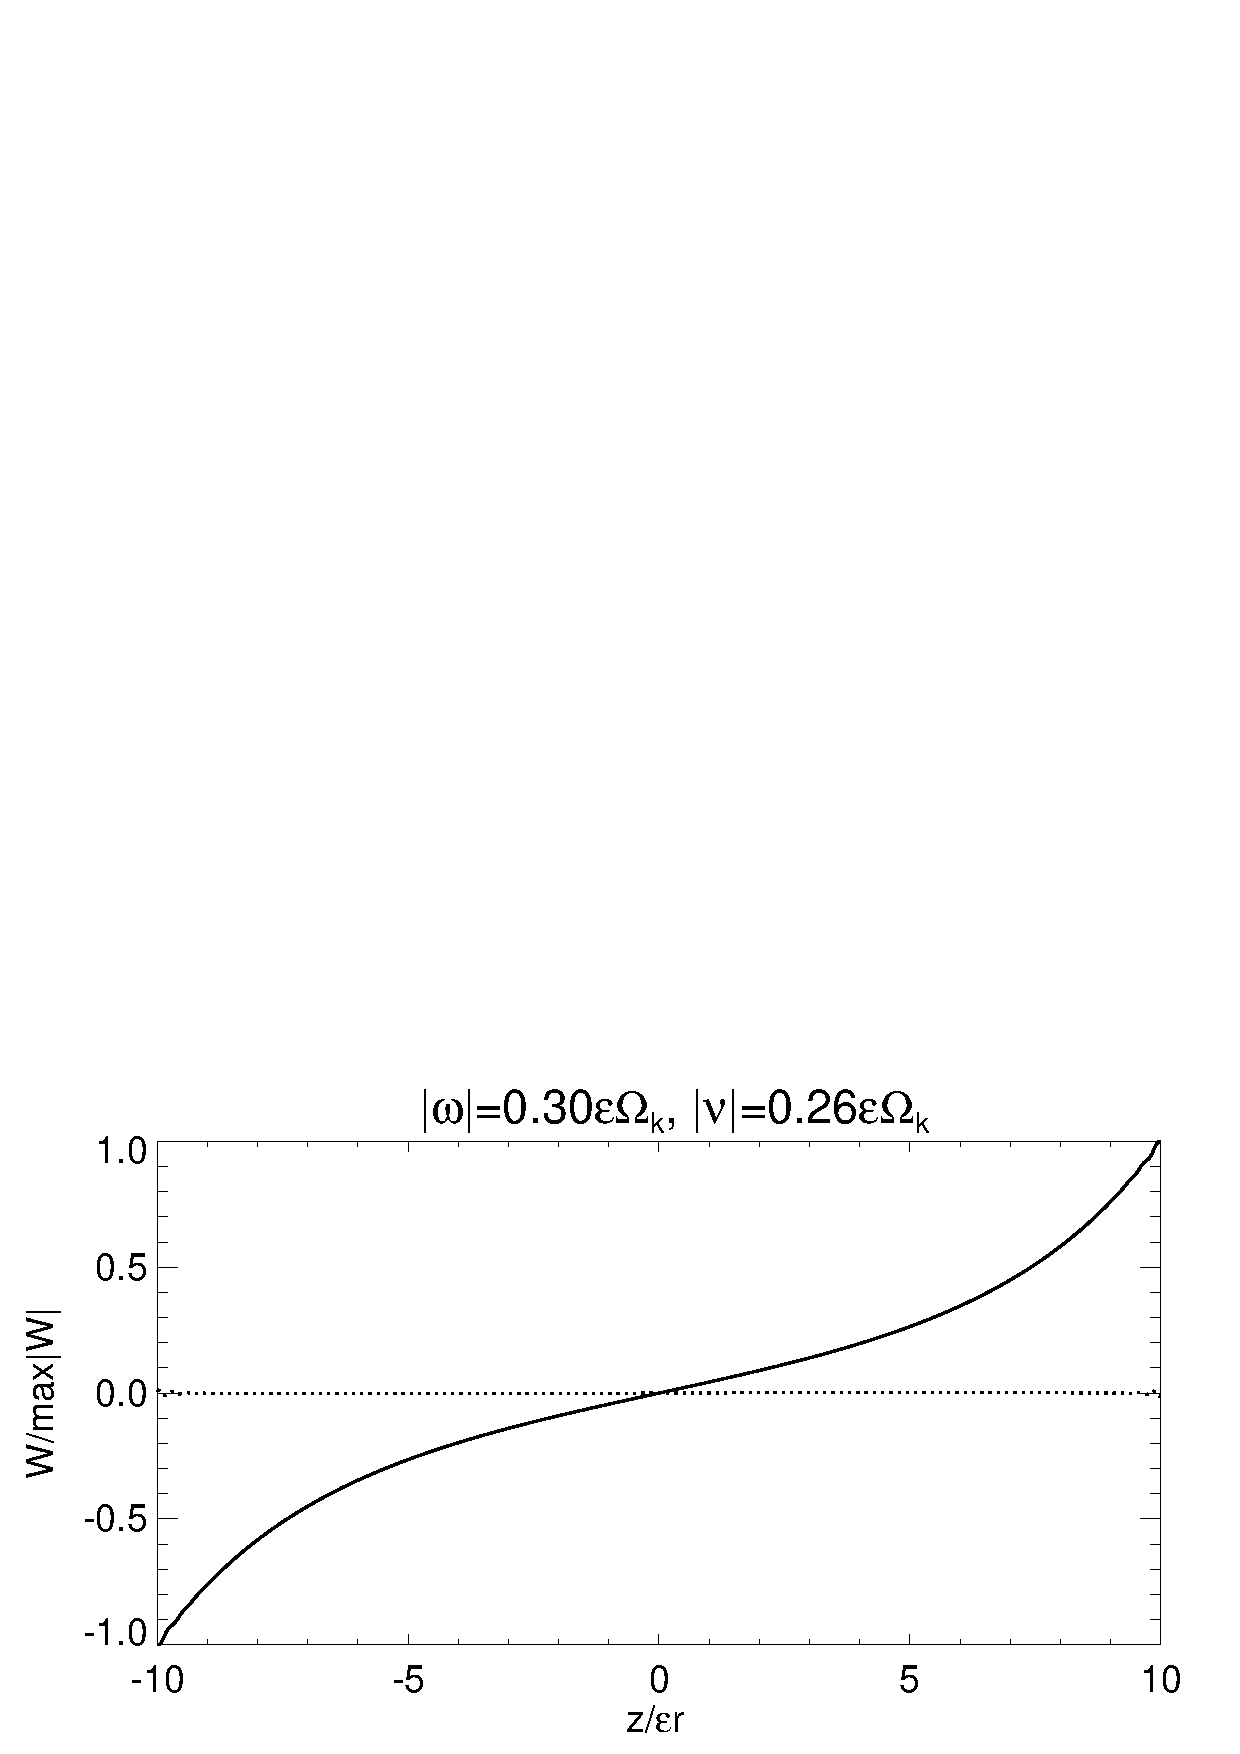
\includegraphics[width=\linewidth]{figures/eigenvector_iso}
  \caption{Eigenfunction of the fundamental VSI,
    corresponding to the bottom-left eigenvalue displayed in
    Fig. \ref{lowfreq_eigen} (smallest $|\sigma|$). The
    solid and dashed lines are $\real W$ and $\imag W$, respectively. 
    \label{lowfreq_eigenfunc}
  }
\end{figure}

\subsection{Stabilization of the VSI by a positive vertical entropy
  gradient}